\chapter{Building the groundwater model}\label{ch:c3}
Raven's HRUs are irregular areas; MODFLOW needs a regular three-dimensional grid. This chapter follows the model builder step by step. It shows which HRUs are coupled, how their polygons are placed on a map
and covered with a grid, and how much of each HRU falls in each cell. It then shows how the layers are built from the land
surface down to bedrock, which MODFLOW files are written, and how MODFLOW solves each step.

\section{From HRUs to a groundwater grid}\label{ch:grid}
\subsection{Which HRUs are coupled}
An HRU is \emph{coupled} when its \cmd{AQUIFER\_PROFILE} in the \cmd{.rvh} file names a profile defined in the
\cmd{.rvp} file. HRUs with \cmd{[NONE]} (or an empty entry) keep Raven's usual behaviour. Disabled HRUs are never
coupled (Raven prints a warning). We write $\mathcal{K}$ for the set of coupled HRUs and $a(k)$ for the aquifer profile of HRU $k$.

Raven checks two rules at start-up:
\begin{itemize}
\item No Raven process may take water \emph{out of} \cmd{GROUNDWATER} in a coupled HRU (MODFLOW owns that water);
Raven stops with an error naming the process.
\item If a process sends water \emph{into} \cmd{GROUNDWATER} in an \emph{uncoupled} HRU, that water leaves the model;
Raven warns so the user can restrict the process with \cmd{:-->Conditional}.
\end{itemize}

\subsection{Map projection}
The HRU polygons are read from a GeoJSON file. GeoJSON coordinates are longitude $\mathrm{lon}$ and latitude $\mathrm{lat}$ in
degrees, which cannot be used directly for areas and distances. Raven converts them to metres with the
\emph{Lambert azimuthal equal-area} projection \cite{snyder1987map}, centred on the average centroid
$(\mathrm{lon}_0,\mathrm{lat}_0)$ of the coupled HRUs, on a sphere of radius $R_\oplus=6\,371\,007.181$ m:
\begin{align}
\kappa &= \sqrt{\frac{2}{1+\sin\mathrm{lat}_0\sin\mathrm{lat}+\cos\mathrm{lat}_0\cos\mathrm{lat}\cos(\mathrm{lon}-\mathrm{lon}_0)}},\\
x &= R_\oplus\,\kappa\cos\mathrm{lat}\,\sin(\mathrm{lon}-\mathrm{lon}_0),\\
y &= R_\oplus\,\kappa\left[\cos\mathrm{lat}_0\sin\mathrm{lat}-\sin\mathrm{lat}_0\cos\mathrm{lat}\cos(\mathrm{lon}-\mathrm{lon}_0)\right].
\end{align}
The reverse conversion (for looking up map values at cell locations) is
\begin{align}
\rho&=\sqrt{x^2+y^2},\qquad c=2\arcsin\frac{\rho}{2R_\oplus},\\
\mathrm{lat}&=\arcsin\!\left(\cos c\sin\mathrm{lat}_0+\frac{y\sin c\cos\mathrm{lat}_0}{\rho}\right),\\
\mathrm{lon}&=\mathrm{lon}_0+\operatorname{atan2}\!\left(x\sin c,\;\rho\cos\mathrm{lat}_0\cos c-y\sin\mathrm{lat}_0\sin c\right).
\end{align}
\begin{plain}
This projection keeps areas correct, which is what matters for water volumes: one square kilometre on the map is one
square kilometre on the ground, anywhere in the model area.
\end{plain}
When the centroid longitudes span more than 180$^\circ$ as written, they are averaged across the antimeridian if that
gives them a smaller span (those west of 0 count 360$^\circ$ more), so that a model across longitude 180$^\circ$ is centred on it (HRUs at 179.998$^\circ$ and
$-179.998^\circ$ give $\mathrm{lon}_0=180^\circ$); the longitudes Raven derives are within $\pm180^\circ$, and a
longitude/latitude raster written beyond $\pm180^\circ$ across the antimeridian is sampled 360$^\circ$ east or west.

\subsection{The grid}
By default a square grid with cell size $\Delta$ (\cmd{:GridCellSize}, default 1\,000 m) covers the rectangle around all
coupled HRUs. Rows are numbered from north to south and columns from west to east. The plan-view cell (a whole column of
layers) is indexed $i$; its lower-left corner is $(x_0+c\Delta,\;y_0+(n_r-1-r)\Delta)$ for row $r$ and column $c$. Rotated
grids, grids refined around rivers and wells, quadtree grids, meshes that follow HRU boundaries and imported cells are
described in Section~\ref{sec:gridtypes}; everything below applies to all of them, with cell $i$ a polygon $\Omega_i$ of area $|\Omega_i|$.

\subsection{Polygon areas}
The area of a polygon with $N_v$ corners $(x_1,y_1),\dots,(x_{N_v},y_{N_v})$ is given by the shoelace formula
\begin{equation}
A=\tfrac12\sum_{v=1}^{N_v}\left(x_vy_{v+1}-x_{v+1}y_v\right),\qquad (x_{N_v+1},y_{N_v+1})=(x_1,y_1).
\end{equation}
The result is positive when the corners run counter-clockwise. Raven orients outer boundaries counter-clockwise and
holes clockwise, so the area of a polygon with holes is simply the sum over all its rings.
\begin{example}[: shoelace formula]
A square from $(0,0)$ to $(2,2)$ km: $\tfrac12[(0\cdot0-2\cdot0)+(2\cdot2-2\cdot0)+(2\cdot2-0\cdot2)+(0\cdot0-0\cdot2)]=\tfrac12(0+4+4+0)=4$ km$^2$.
\end{example}

\subsection{How much of each HRU lies in each cell}\label{sec:linkage}
For every HRU polygon $P_k$ and every cell $\Omega_i$ it touches, Raven cuts the polygon to the cell rectangle with
the Sutherland--Hodgman clipping algorithm \cite{sutherland1974clip} and measures the area of what remains:
\begin{equation}
A_{k,i}=\left|P_k\cap\Omega_i\right| .
\end{equation}
For rectangular cells (regular and quadtree grids) the polygon is clipped by the cell rectangle; for convex cells (HRU
meshes) by the cell polygon; a concave imported cell is split into triangles and clipped by each. The clipping works one
cell edge at a time: walking around the polygon, it keeps the corners that are inside the edge
and adds a new corner wherever the polygon crosses the edge. After four edges, what is left is the part of the polygon
inside the cell; the shoelace formula gives its area. (This gives the correct area even for concave polygons.)

\begin{example}[: overlap areas]
An HRU of 10 km$^2$ lies over three 2~km cells, covering 4.0, 3.5 and 2.5 km$^2$ of them. Its overlaps are
$A_{k,1}=4.0$, $A_{k,2}=3.5$, $A_{k,3}=2.5$ km$^2$, and the fractions of the HRU in each cell are 0.40, 0.35 and 0.25.
Every flow from this HRU to the grid is split 40/35/25.
\end{example}

\subsection{Active cells and their profile}
A column is \emph{active} when the coupled HRUs cover at least a fraction $f_{\min}$ (\cmd{:MinCellCoverage}, default
0.25) of it:
\begin{equation}
A^{\mathrm{cov}}_i=\sum_{k\in\mathcal{K}}A_{k,i}\ \ge\ f_{\min}\,|\Omega_i| .
\end{equation}
An active column takes the profile of the HRU with the largest overlap (the \emph{dominant} HRU),
$a(i)=a\!\left(\arg\max_k A_{k,i}\right)$. Fluxes still use the exact overlaps, so a column shared by two HRUs receives
water from both.

The table of overlaps $A_{k,i}$ over active columns is called the \emph{linkage}. It is the single source of truth for
moving water between HRUs and cells in both directions (Sections~\ref{ch:recharge}--\ref{ch:stores}).

\begin{watch}
The polygon area of an HRU need not equal its \cmd{AREA} in the \cmd{.rvh} file (Raven prints a warning when they
differ by more than 5\%). This does not break the water balance: volumes are always computed from the \cmd{.rvh} area
and split by overlap \emph{fractions}.
\end{watch}

\subsection{The linkage cache}
Computing the linkage requires reading and clipping every polygon. The result is saved in \cmd{<output>/mf6/linkage.cache}
(or the file named by \cmd{:LinkageCache}). The cache is labelled with a fingerprint (an FNV-1a hash) of the GeoJSON
file together with the ID field, the cell size and the list of coupled HRUs; if any of these change, Raven recomputes
the linkage. Numbers are written with 17 significant digits, so a run that reads the cache gives exactly the same
results as one that computed it.

\begin{figure}[!htbp]\centering
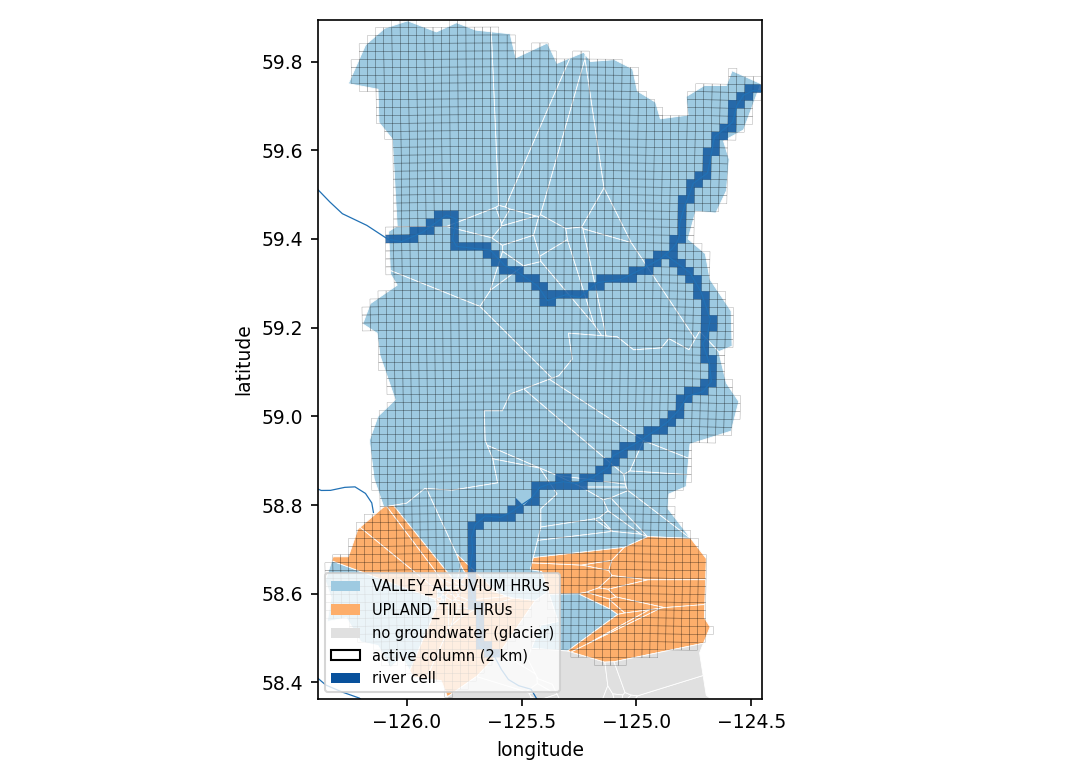
\includegraphics[width=0.9\linewidth]{figures/fig_grid_liard.png}
\caption{Liard example: coupled HRUs (colour = aquifer profile), active 2~km columns and river cells.}\label{fig:grid}
\end{figure}

\section{From one HRU to its cells: a complete example}
\begin{figure}[!htbp]\centering
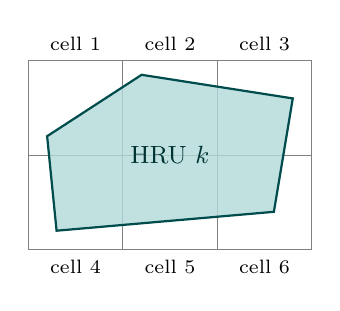
\begin{tikzpicture}[x=1.2cm,y=1.2cm]
\foreach \x in {0,1,2,3} \draw[gray] (\x,0) -- (\x,2);
\foreach \y in {0,1,2} \draw[gray] (0,\y) -- (3,\y);
\fill[teal!30,opacity=0.8] (0.3,0.2) -- (2.6,0.4) -- (2.8,1.6) -- (1.2,1.85) -- (0.2,1.2) -- cycle;
\draw[teal!60!black,thick] (0.3,0.2) -- (2.6,0.4) -- (2.8,1.6) -- (1.2,1.85) -- (0.2,1.2) -- cycle;
\node[font=\scriptsize] at (0.5,2.18) {cell 1}; \node[font=\scriptsize] at (1.5,2.18) {cell 2}; \node[font=\scriptsize] at (2.5,2.18) {cell 3};
\node[font=\scriptsize] at (0.5,-0.18) {cell 4}; \node[font=\scriptsize] at (1.5,-0.18) {cell 5}; \node[font=\scriptsize] at (2.5,-0.18) {cell 6};
\node[font=\small,teal!40!black] at (1.5,1.0) {HRU $k$};
\end{tikzpicture}
\caption{An HRU polygon over six grid cells. Clipping gives its area in each cell.}\label{fig:hrucells}
\end{figure}
\begin{example}[: an HRU through the whole chain]
Suppose the HRU in Figure~\ref{fig:hrucells} has an \cmd{.rvh} area of 3.2 km$^2$, 2 km cells, and clipping gives overlaps (km$^2$)
0.45, 0.55, 0.30 in cells 1--3 and 0.60, 0.85, 0.45 in cells 4--6 (sum 3.20).
\begin{enumerate}
\item \emph{Activation.} If other coupled HRUs fill the rest of these cells, all six have coverage above 25\% and are active.
\item \emph{Recharge.} Raven's percolation puts 1.5 mm into \cmd{GROUNDWATER}: $V=0.0015\times3.2\times10^6=4\,800$ m$^3$.
Cell 5 receives $4\,800\times0.85/3.20=1\,275$ m$^3$, i.e.\ $1\,275/4\times10^6=0.32$ mm over the whole cell (plus whatever other
HRUs deliver).
\item \emph{Seepage back.} If cell 5 seeps 10\,000 m$^3$ in the day and our HRU covers 0.85 of the 4 km$^2$ covered by all
HRUs in that cell, the HRU receives $10\,000\times0.85/4.0=2\,125$ m$^3$, i.e.\ $2\,125/3.2\times10^6\times1000=0.66$ mm in its lowest soil layer.
\item \emph{Water-table depth in the outputs.} \cmd{GWHRUState.csv} reports the overlap-weighted mean head of the six cells.
\end{enumerate}
\end{example}

\section{Preparing the geometry}
\subsection{What the HRU GeoJSON must contain}
A \cmd{FeatureCollection} of \cmd{Polygon} or \cmd{MultiPolygon} features in longitude/latitude (EPSG:4326), or in the
projection of \cmd{:InputCRS} (Section~\ref{sec:inputcrs}), each with a property holding the HRU ID of the \cmd{.rvh} file. Holes are allowed. Several features may share an ID (their areas add up).
\par\noindent\begin{minipage}{\linewidth}
\begin{lstlisting}
{"type":"FeatureCollection","features":[
 {"type":"Feature","properties":{"HRU_ID":2736},
  "geometry":{"type":"Polygon","coordinates":[[[-124.91,59.22],[-124.80,59.22],
              [-124.80,59.30],[-124.91,59.30],[-124.91,59.22]]]}} ]}
\end{lstlisting}
\end{minipage}\par\smallskip
Only HRUs with an \cmd{AQUIFER\_PROFILE} need polygons; others may be present and are ignored.
Every GeoJSON file Raven reads (HRUs, grids, boundaries, refinement features) is read as strict JSON: a coordinate must be a
finite JSON number: a string such as \cmd{"-124.91"}, \cmd{null}, \cmd{true}, \cmd{NaN} or \cmd{Infinity} stops the run,
naming the file, the feature, the ring and the vertex, and so does a position that is not an array of at least two
numbers (coordinates nested one level too deep or too shallow for the geometry type, a vertex \cmd{[1]}); hexadecimal
numbers and numbers with leading zeros are not JSON, and neither is text after the root object (the file is refused as
invalid JSON, naming the line and column). \cmd{NaN}, \cmd{Infinity} and \cmd{-Infinity} are read in the attributes, as
GDAL and Python's \cmd{json} write them, and \cmd{\textbackslash uXXXX} escapes are read as the characters they stand for,
so a field name such as \cmd{H\"ohe\_ID} matches. An ID field must hold a whole number, or a string that holds exactly
one (\cmd{7}, \cmd{7.0}, \cmd{"7"}, \cmd{" 7"}, \cmd{"7.0"}); \cmd{null}, \cmd{true}, a fraction or other text stops the run
(features of other geometry types than the file's are skipped before their ID is read), naming the file, the
feature and the value. A feature without a \cmd{"properties"} member stops the run where an ID field is read (a boundary
or refinement file needs none).
\subsection{Raster maps}\label{sec:rasters}
\cmd{:LandSurface} and \cmd{:BedrockSurface} take an ESRI ASCII grid or a GeoTIFF file (Section~\ref{sec:geotiff}), in
longitude/latitude or in the projection of \cmd{:InputCRS} (Section~\ref{sec:inputcrs}). An ESRI ASCII grid, for example:
\par\noindent\begin{minipage}{\linewidth}
\begin{lstlisting}
ncols 125
nrows 115
xllcorner -126.6
yllcorner 58.1
cellsize 0.02
NODATA_value -9999
 612.3 615.9 ...
\end{lstlisting}
\end{minipage}\par\smallskip
Values are interpolated bilinearly between raster cell centres, ignoring no-data cells; each model cell takes the mean of
$5\times5$ such samples. Points more than half a raster cell beyond the map's edge (one cell beyond the outermost cell centres) count as no-data. A grid without a
\cmd{NODATA\_value} line has no no-data value, as GDAL reads it: every number is an elevation (Raven warns when such a grid
holds $-9999$, which often marks missing data). The header keys may come in any order and case; \cmd{xllcenter} and
\cmd{yllcenter} give the centre of the lower-left cell instead of its corner; rectangular cells are given, as GDAL writes
them, by \cmd{dx} and \cmd{dy} instead of \cmd{cellsize}; \cmd{NODATA\_value nan} marks no-data cells written as
\cmd{nan}; a UTF-8 byte-order mark before the header and a DOS end-of-file mark (Ctrl-Z) after the values are ignored. The grid must hold exactly \cmd{ncols}$\times$\cmd{nrows} values: an unknown header key, a key given twice or both
\cmd{xllcorner} and \cmd{xllcenter} (or both \cmd{y} keys), a header value or a
cell value that is not a number, fewer values or more values (a wrong \cmd{ncols} would otherwise wrap the rows) stop
the run with a message naming the problem.

A raster that gives no value for any active column (all 25 samples of every column no-data or off the map) stops the run:
it is a map of another area, has a wrong corner, or is in another projection than \cmd{:InputCRS}. The message gives the
raster's extent and the extent of the active columns, both in the raster's coordinates. A raster that misses only some
columns gives a warning with their number; those columns take the area-weighted HRU \cmd{ELEVATION} (DEM) or lie
\cmd{DEFAULT\_BEDROCK\_DEPTH} below the land surface (bedrock). A raster may have at most 50 million cells: resample a
finer one (a few raster cells per model cell are enough).

\subsubsection{GeoTIFF files}\label{sec:geotiff}
A raster file whose name ends in \cmd{.tif}, \cmd{.tiff} or \cmd{.gtiff} (in any case) is read as GeoTIFF by Raven's own reader; no GDAL
or other library is needed. The values and their georeferencing are then sampled exactly as those of an ESRI ASCII grid:
a GeoTIFF and an ESRI ASCII grid with the same values give the same model.
\begin{center}
\begin{tabular}{P{0.25\linewidth}P{0.68\linewidth}}
\toprule\hdr Item & Supported\\\midrule
file & classic TIFF and BigTIFF, little- and big-endian; the first image of the file (overviews are ignored); at most 1~GB\\
units & coordinates in metres (projections) or degrees from Greenwich, elevations in metres: units keys, a projected code
in other units, a prime meridian (by code, by its longitude or by the datum), a vertical coordinate system in feet or a
band unit that is not a metre form (Table~\ref{tab:bandunits}) stop the run; a vertical system Raven does not know
gives a warning (read as metres)\\
scale and offset & GDAL's band \cmd{SCALE} and \cmd{OFFSET} (tag \cmd{GDAL\_METADATA}, items with GDAL's role
\cmd{scale}, \cmd{offset}, \cmd{unittype}; items of the same name without it are ordinary metadata, as for GDAL) are
applied, value $\times$ scale $+$ offset, as GDAL's \cmd{-unscale} and GIS programs show the values; no-data pixels, and
values beyond the range of a double, are no-data; a \cmd{GDAL\_METADATA} tag over 16~MB stops the run\\
side file & GDAL's side file \cmd{<raster>.aux.xml} (written for example with \cmd{-co PROFILE=GeoTIFF} or
\cmd{BASELINE}, or when metadata are set on a file opened read-only) is read as GDAL reads it, before the file's own
metadata: in its \cmd{PAMRasterBand band="1"}, a \cmd{Scale} or an \cmd{Offset} replaces both of the file's (the other
is then 1 or 0), a \cmd{UnitType} replaces the band unit, and a \cmd{NoDataValue} replaces \cmd{GDAL\_NODATA}. Raven reads
the side file, and \cmd{GDAL\_METADATA}, only in the form GDAL writes them (its layout, attributes in double quotes, one
\cmd{PAMRasterBand} per band, GDAL's escapes, and the comments, literals such as \cmd{<!DOCTYPE ...>}, processing
instructions and mixed text GDAL writes in an \cmd{xml:} metadata domain, which are read past); one in any other form that names a band or a band value (\cmd{PAMRasterBand},
\cmd{Scale}, \cmd{Offset}, \cmd{UnitType}, \cmd{NoDataValue}) stops the run (``rewrite it with GDAL'': \cmd{gdal\_translate}
or \cmd{gdal\_edit.py}), and one that names none is ignored, as GDAL takes no band value from it; a file with CRLF line ends is not
in that form (the message says so); a GeoTIFF's side file that holds georeferencing (\cmd{GeoTransform}, \cmd{SRS} or \cmd{GCPList},
which GDAL may take in place of the raster's own), a value that is not a number or a side file over 16~MB stops the run. An ESRI ASCII grid's side file is read the same way (its \cmd{Scale},
\cmd{Offset} and \cmd{UnitType}; GDAL keeps the grid's \cmd{NODATA\_value}, and ignores a \cmd{GeoTransform} or \cmd{SRS} there, taking
the grid's header and its \cmd{.prj}, as Raven does), so a GeoTIFF and the ESRI ASCII grid GDAL makes
of it give the same model. Georeferencing kept only in the side file (\cmd{BASELINE}) is not read: such a file stops as having no georeferencing\\
layout & strips or tiles\\
compression & none, LZW, DEFLATE (codes 8 and 32946) and PackBits\\
predictor & none, horizontal differencing (2) and floating-point (3), with LZW and DEFLATE\\
values & one band (one sample per pixel, grey scale); unsigned and signed integers of 8, 16, 32 and 64 bits, floating
point of 32 and 64 bits\\
georeferencing & north-up: \cmd{ModelPixelScale} with \cmd{ModelTiepoint}, or a \cmd{ModelTransformation} without rotation
or shear; pixels may be rectangular\\
pixel position & \cmd{PixelIsArea} (the default): the tie point is the corner of the pixel; \cmd{PixelIsPoint}: the tie
point is the centre of the pixel, so the raster's corner lies half a pixel up and left of it (as GDAL reads it)\\
no-data & the \cmd{GDAL\_NODATA} tag (a 32-bit float raster compares at 32-bit precision; \cmd{nan} allowed), and a GDAL
internal mask (1 or 8 bits; mask 0 is no-data; looked for among the first 4\,096 image directories; a damaged
chain of directories after the raster gives a warning and the raster without its mask); without either every value is valid, as GDAL reads it. NaN and infinite
values are always no-data\\
\bottomrule
\end{tabular}
\end{center}
The run stops with a message naming the file and the reason for: other compressions (JPEG, ZSTD, LZMA, LERC, WebP,
\dots), more than one band, a palette or colour image, other bit depths (1, 12 or 16-bit floating point, complex values),
a rotated, sheared or south-up raster, control points without a pixel size, no georeferencing, geocentric coordinates,
bits stored in reverse order (\cmd{FillOrder} 2), projected coordinates or elevations in other units than metres
(\cmd{ProjLinearUnitsGeoKey}, \cmd{GeogLinearUnitsGeoKey}, \cmd{VerticalUnitsGeoKey}) or longitude/latitude in other units
than degrees, a geographic code or key with a prime meridian other than Greenwich (for example EPSG:4801, Bern), also
when the prime meridian is given only by its longitude (\cmd{GeogPrimeMeridianLongGeoKey}, as GDAL writes a user-defined
longitude/latitude system such as \cmd{+pm=paris}) or by the datum (\cmd{GeogGeodeticDatumGeoKey}, for example 6801), a
projected code whose coordinates are in feet or other units when the file has no \cmd{ProjLinearUnitsGeoKey} (for example
EPSG:2227, California zone 3 in US survey feet), a band unit (\cmd{UNITTYPE} in \cmd{GDAL\_METADATA}, or
\cmd{UnitType} in the side file) that is not a metre form, a band \cmd{SCALE} of 0, a
vertical coordinate system in feet (for example EPSG:4269+6360, NAVD88 in US survey feet), an internal mask Raven cannot
read, a truncated or corrupt file or a decompression error, and a file over 1~GB, 50 million pixels, or strips or tiles
covering more than 200 million pixels. Raven is stricter than GDAL in a few rare cases: a negative pixel height
(\cmd{ModelPixelScale}, which GDAL reads north-up by default) is refused, a \cmd{ModelTiepoint} tag of more than 4\,096
values is taken as no georeferencing, and a \cmd{GDAL\_NODATA} text longer than 256 characters is ignored.

\paragraph{Band unit.} GDAL's band unit (\cmd{UNITTYPE} in \cmd{GDAL\_METADATA}, or \cmd{UnitType} in the side file;
set with \cmd{gdal\_edit.py -units}) is free text, so Raven's rule is closed: the raster is read as metres only when the
whole text, normalised, is a metre form of Table~\ref{tab:bandunits}: a metre word, symbol or abbreviation, alone or followed
by one listed vertical datum (\cmd{m MSL}, \cmd{m, AHD}, \cmd{m (NAVD88)}, \cmd{m(NAVD88)}, \cmd{m-NAVD88},
\cmd{m NAVD88 GEOID18}, \cmd{meters (EGM2008 geoid)}, \cmd{m above sea level}, fused \cmd{mAHD}, \cmd{msnm}, \cmd{m.s.n.m.}), a metre form in brackets after a metre word (\cmd{meter (m)},
\cmd{metre (EPSG:9001)}), or a metre form after a quantity, in brackets or after \cmd{in} (\cmd{elevation (m)},
\cmd{Elevation [m]}, \cmd{height in metres}, \cmd{height above ellipsoid (m)}, \cmd{H\"ohe (m)}, \cmd{Elevation\_m}). Normalising reads full-width characters as
ASCII and no-break and ideographic spaces as blanks, trims the blanks and reads a run of them as one, lowers the case (ASCII,
Latin-1, Latin Extended-A, Greek, whose accents are also removed, and Cyrillic) and removes surrounding brackets: \cmd{m},
\cmd{m.}, \cmd{(m)}, \cmd{[metres]}, \cmd{Meters}, \cmd{MASL}, \cmd{m a.s.l.}, \cmd{m\"uNN}, \cmd{Meter \"uber NN},
\cmd{$\mu\acute{\epsilon}\tau\rho\alpha$}, the same in capitals without accents, a full-width \cmd{m}, \cmd{EPSG:9001} are
metres. A raster without a band unit is read as metres (empty brackets, \cmd{()} or \cmd{[]}, are a text). Any other text
stops the run with a message that names the text (bytes that are not UTF-8 shown as \cmd{\textbackslash xNN}), of one of
three kinds:
\begin{itemize}
\item a text with another length unit and no metre (the second row of the table: \cmd{ft}, \cmd{US survey foot},
\cmd{Zentimeter}, \cmd{km}, \cmd{EPSG:9002}, also \cmd{EPSG 9002} and \cmd{EPSG: 9003}, feet fused with a datum such as
\cmd{ftMSL}, \cmd{ftNAVD88} or \cmd{usftNGVD29}, the ESRI unit names \cmd{Link\_Clarke} or \cmd{Rod\_US}), or another length named with its metre conversion (\cmd{ft (0.3048 m)}, \cmd{M (feet)}): ``its elevations are
in \dots''; convert the values to metres and set the unit
(\cmd{gdal\_calc.py}, then \cmd{gdal\_edit.py -units m});
\item a scaled metre: a part or multiple (\cmd{m (in thousands)}, \cmd{tenths of a metre}, \cmd{m (in 1000s)}), a number with a
factor sign or word (\cmd{m*0.1}, \cmd{Meter (x0.1)}, \cmd{m (scaled by 0.1)}, \cmd{0.1 of a metre}, \cmd{Meter (Faktor 0,1)},
\cmd{units of 0.1 m}, \cmd{m\^{}2}), a power of ten or an ordinal (\cmd{m 1e-2}, \cmd{m E-2}, \cmd{100ths of a metre}), or a number
and a metre form as the whole text (\cmd{0.1 m}, \cmd{1000 m}, \cmd{1e-2 m}, \cmd{.1 m}): the values are not plain metres; write them unscaled, or give
the scale as the band's scale and offset (\cmd{gdal\_edit.py -scale 0.1 -units m});
\item any other text (\cmd{m (Admiralty datum)}, \cmd{hydraulic head}, \cmd{m/s}, \cmd{5 km grid, elevation in m}, \cmd{m
(NAVD 1988)}): if the elevations are in metres (after the band scale and offset), state it by writing \cmd{METRES} (or
\cmd{METERS}) after the file name, otherwise convert as above:
\begin{verbatim}
:LandSurface   dem.tif   METRES
\end{verbatim}
(\cmd{:BedrockSurface} likewise).
\end{itemize}
\cmd{METRES} is the user's statement that the values are metres, for a text Raven cannot place: it does not lift the
first two kinds (a recognised other length or scaled metre stops also with it). With \cmd{METRES} every run writes a
warning that names the file's own unit text, also for a metre form or no unit (``read as metres because METRES follows the
file name \dots; the file's own band unit is \dots''), so that a wrong statement shows.
\begin{table}[!htbp]\centering
\caption{Band units: the metre forms read as metres (with their datums and quantities), and the other lengths named in the stop message.}\label{tab:bandunits}\small
\begin{tabularx}{\linewidth}{P{0.2\linewidth}Y}\toprule\hdr
Class & Forms (the whole text, normalised)\\\midrule
metre (read as metres) & the metre written out: \cmd{metre}, \cmd{metres}, \cmd{meter}, \cmd{meters}, \cmd{metern},
\cmd{m\`etre(s)}, \cmd{m\'eter}, \cmd{m\'eterben}, \cmd{metro(s)}, \cmd{metri}, \cmd{metr}, \cmd{metra}, \cmd{metry},
\cmd{metr\'ow}, \cmd{metrach}, \cmd{metrami}, \cmd{metrze}, \cmd{metrem}, \cmd{metr\r{u}}, \cmd{metrech}, \cmd{metru},
\cmd{metrin}, \cmd{metri\"a}, \cmd{metrit}, the metre in Cyrillic (with its endings), Greek, Chinese,
Japanese and Korean; the symbol \cmd{m} (also its Cyrillic letter); \cmd{masl}, \cmd{m asl},
\cmd{m a.s.l.}, \cmd{m.a.s.l.}, \cmd{mamsl}, \cmd{m amsl}, \cmd{m a.m.s.l.}, \cmd{moh}, \cmd{m.o.h.}, \cmd{m\"oh},
\cmd{m \"o.h.}, \cmd{m.\"o.h.}, \cmd{m o.h.}, \cmd{mt}, \cmd{mts}, \cmd{mtr}, \cmd{mtrs}, \cmd{m\"u}, \cmd{m\"uNN}, \cmd{m \"u. NN}, \cmd{m \"u.NN}, \cmd{m \"u. M.}, \cmd{m \"u.M.}, \cmd{m.}, and the Cyrillic metre of the
Baltic system (m BS, written together or apart); \cmd{EPSG:9001}, \cmd{EPSG::9001}, \cmd{EPSG 9001}, \cmd{urn:ogc:def:uom:EPSG::9001}, \cmd{http://www.opengis.net/def/uom/EPSG/0/9001}\\
vertical datums (after a metre form, also with a comma, \cmd{;}, \cmd{/}, \cmd{-} or \cmd{\_}, in brackets, or fused to \cmd{m} or \cmd{m.}) & \cmd{MSL}, \cmd{AMSL},
\cmd{ASL}, \cmd{a.s.l.}, \cmd{a.m.s.l.}, \cmd{above sea level}, \cmd{above mean sea level}, \cmd{AHD}, \cmd{AOD}, \cmd{ODN},
\cmd{NAP}, \cmd{+NAP}, \cmd{TAW}, \cmd{NN}, \cmd{NHN}, \cmd{\"u. NN}, \cmd{\"u.NN}, \cmd{\"uber NN}, \cmd{\"u. NHN},
\cmd{\"u.NHN}, \cmd{\"uber NHN}, \cmd{\"u. M.}, \cmd{NN2000}, \cmd{RH2000}, \cmd{DVR90}, \cmd{NAVD88}, \cmd{NAVD 88},
\cmd{NGVD29}, \cmd{NGVD 29}, \cmd{CGVD2013}, \cmd{CGVD28}, \cmd{EGM96}, \cmd{EGM2008}, \cmd{s.l.m.}, \cmd{slm},
\cmd{n.p.m.}, \cmd{npm}, \cmd{s.n.m.}, \cmd{snm}, \cmd{n. m.}, \cmd{n.m.}, \cmd{ellipsoidal}, \cmd{above (the) ellipsoid};
\cmd{s. n. m.}, \cmd{EGM08}, \cmd{OD}, \cmd{MLLW}, \cmd{MLW}, \cmd{MHW}, \cmd{MHHW}, \cmd{LAT}, \cmd{HAE}, \cmd{orthometric},
\cmd{NGF}, \cmd{IGN69}, \cmd{N2000}, \cmd{NZVD2016}, \cmd{T.P.}, \cmd{(the) WGS84 ellipsoid}; \cmd{NAVD}, \cmd{NGVD},
\cmd{EVRF2000}, \cmd{EVRF2007}, \cmd{DHHN92}, \cmd{DHHN2016}, \cmd{NHN2016}, \cmd{\"u. NHN2016}, \cmd{LN02}, \cmd{\"u. A.},
\cmd{Bpv}, \cmd{n. m. Bpv}, \cmd{NGF-IGN69}, \cmd{t.o.v. NAP}, \cmd{N60}, \cmd{DNN}, \cmd{AHD71}, \cmd{CD}, \cmd{chart datum},
\cmd{OSGM15}, \cmd{Ordnance Datum}, \cmd{geoid}, \cmd{WGS84}, \cmd{TP}; each may end in \cmd{geoid} or a geoid model
(\cmd{m NAVD88 GEOID18}, \cmd{m NAVD88 (GEOID12B)}), follow \cmd{above} or \cmd{over} (\cmd{m above MSL}) and have a blank before its year (\cmd{RH 2000}, \cmd{EGM 96}); a dotted abbreviation of a
metre form or datum may lack its final dot (\cmd{m a.s.l}, \cmd{moh.} with it)\\
quantities (before a metre form in brackets or after \cmd{in}) & \cmd{elevation(s)}, \cmd{height(s)}, \cmd{altitude},
\cmd{elevation / height above (mean) sea level}, \cmd{height above ellipsoid}, \cmd{height\_above\_ellipsoid},
\cmd{ellipsoidal height}, \cmd{orthometric height}, \cmd{elev}, \cmd{z}, \cmd{DEM}, \cmd{DTM}, \cmd{DSM}, and in the languages
of the metre words \cmd{H\"ohe}, \cmd{altitud}, \cmd{altura}, \cmd{cota}, \cmd{hauteur}, \cmd{\'el\'evation}, \cmd{quota},
\cmd{altezza}, \cmd{altitudine}, \cmd{hoogte}, \cmd{wysoko\'s\'c}, \cmd{v\'y\v{s}ka}, \cmd{nadmo\v{r}sk\'a v\'y\v{s}ka},
\cmd{magass\'ag}, \cmd{korkeus}, \cmd{h\"ojd}, \cmd{h\o{}yde}, \cmd{h\o{}jde}, \cmd{\^in\u{a}l\c{t}ime}, the height in Cyrillic and Greek;
also before a comma (\cmd{Elevation, m}) or joined by \cmd{\_} (\cmd{Elevation\_m})\\
another length (named in the message; \cmd{METRES} does not apply) & a text with one of these and no metre form among its
words: feet, inches, yards, miles, fathoms, chains and furlongs in English and other languages and case forms (\cmd{ft},
\cmd{foot}, \cmd{feet}, \cmd{fasl}, \cmd{inch(es)}, \cmd{yard(s)}, \cmd{mile(s)}, \cmd{pie(s)}, \cmd{pied(s)}, \cmd{voet},
\cmd{Fu\ss}, \cmd{F\"u\ss e}, \cmd{stopa}, \cmd{stopach}, \cmd{st\'op}, \cmd{jalka}, \cmd{l\'ab}, \cmd{l\'abban}, \cmd{Zoll},
\cmd{pulgada(s)}, \cmd{Meile(n)}, \cmd{polegada(s)}, \cmd{milha(s)}, \cmd{jarda(s)}, \cmd{cal}, \cmd{cale}, \cmd{mil},
\cmd{jardy}, \cmd{palce}, \cmd{m\'ile}, \cmd{h\"uvelyk}, \cmd{m\'erf\"old}, \cmd{tuuma}, \cmd{maili}, \cmd{jaardi}, \cmd{tum},
\cmd{tomme}, \cmd{picior}, \cmd{inci}, \cmd{yarzi}, \cmd{milles}, \cmd{verges}, \cmd{iarde}, \cmd{vara(s)}, the fathom as
\cmd{braza(s)}, \cmd{bra\c{c}a(s)}, \cmd{brasse(s)}, \cmd{toise(s)}, \cmd{Faden}, \cmd{Klafter}, \cmd{vadem}, \cmd{famn},
\cmd{favn}, and in Cyrillic, Greek, Chinese, Japanese and Korean, with the verst and arshin and the Chinese and Japanese
chi, shi chi, cun, zhang, li and ken); \cmd{micron(s)}, \cmd{rod(s)}, \cmd{perch(es)}, \cmd{league(s)},
\cmd{kft}; the ESRI unit names \cmd{Link\_}\dots, \cmd{Chain\_}\dots, \cmd{Rod\_}\dots; feet fused with a qualifier
(\cmd{ftUS}, \cmd{usft}, \cmd{SurveyFeet}) or a datum, its year kept (\cmd{ftMSL}, \cmd{ftNAVD88}, \cmd{ftNAVD 88},
\cmd{usftNGVD29}, also as a word of a longer text: \cmd{elevation (ftNAVD88)}); the metre's multiples and parts as symbols (\cmd{km}, \cmd{cm}, \cmd{mm},
\cmd{dm}, \cmd{nm}, \cmd{$\mu$m}, also Cyrillic) or with an SI prefix joined to a metre word or right before one
(\cmd{kilometres}, \cmd{Kilo Meter}, \cmd{Zentimeter}, \cmd{dec\'imetros}, \cmd{quil\'ometros}, \cmd{milli-metres}, and
the prefixed metres of Chinese, Japanese and Korean, also with a blank between the prefix and the metre);
\cmd{in}, \cmd{ch}, \cmd{mi}, \cmd{fath}, \cmd{link(s)}, \cmd{dam}, \cmd{hm} as the whole text (or after \cmd{us},
\cmd{ind}, \cmd{int}, \cmd{intl}); EPSG length codes other than 9001 as the whole text (\cmd{EPSG:9002},
\cmd{urn:ogc:def:uom:EPSG::9036}; as part of a longer text such codes, several of which also name coordinate systems,
are not read as units)\\\bottomrule
\end{tabularx}
\end{table}

A GeoTIFF without \cmd{GDAL\_NODATA} (for example one converted from an ESRI ASCII grid without its \cmd{NODATA\_value})
holds no no-data value: every value is an elevation, also $-9999$. When such a file holds $-9999$, the lowest or highest
32- or 64-bit float or, for signed integers, the type's minimum, Raven warns with the number of pixels of each value; if
they mark missing data, declare the no-data value (\cmd{gdal\_translate -a\_nodata -9999 in.tif out.tif}). A GeoTIFF that GDAL
writes with its default options (\cmd{gdal\_translate}, \cmd{gdalwarp}, QGIS export), uncompressed or with
\cmd{COMPRESS=LZW}, \cmd{DEFLATE} or \cmd{PACKBITS}, is read as it is; otherwise convert it, for example
\cmd{gdal\_translate -b 1 -co COMPRESS=DEFLATE in.tif dem.tif}.

\paragraph{Coordinate system of a GeoTIFF.} The EPSG code of the GeoTIFF keys (\cmd{ProjectedCSTypeGeoKey} of a projected
raster, \cmd{GeographicTypeGeoKey} of a geographic one) is checked against the run:
\begin{itemize}
\item a geographic code (longitude/latitude, any datum) is accepted without \cmd{:InputCRS} and refused with it;
\item a projected code needs \cmd{:InputCRS}: the same code, or a built-in code or parameters giving the same projection;
another built-in projection, or another EPSG code given as \cmd{:InputCRS}, is refused;
\item a projected code that is not built in cannot be compared with \cmd{:InputCRS} given by its parameters (\cmd{TMERC},
\cmd{ALBERS}, \cmd{LCC}): the file is read in the \cmd{:InputCRS} coordinates, with a warning; under \cmd{:InputCRS}
given as a code (\cmd{EPSG:}\emph{n} or \cmd{ESRI:102001}) it is refused. Without \cmd{:InputCRS} the message asks for
\cmd{:InputCRS EPSG:}\emph{n} when the code is built in, otherwise for the projection's parameters;
\item a user-defined coordinate system (code 32767) or none at all says nothing: the file is treated as an ESRI ASCII grid,
whose extent alone is checked (the longitude/latitude range without \cmd{:InputCRS}, ``looks like longitude/latitude''
with it).
\end{itemize}
The message of a refused file names the file, the code found and the coordinate system expected.
\subsection{Projected input files (\texttt{:InputCRS})}\label{sec:inputcrs}
Most GIS data are projected (UTM, Albers, Lambert). Instead of reprojecting them to longitude/latitude, give their
projection once in the \cmd{.rvg} file:
\begin{lstlisting}
:InputCRS EPSG:32610                                   # UTM zone 10 N (WGS84)
:InputCRS ALBERS 50 58.5 45 -126 1000000 0 GRS80       # or by parameters (here BC Albers, EPSG:3005)
\end{lstlisting}
The grammar is that of \cmd{:MF6CRS} (Section~\ref{sec:mf6crs}): the EPSG codes 326xx and 327xx (UTM, WGS84), 269xx (UTM, NAD83),
3005, 5070, 3978, 3347 and ESRI:102001, or \cmd{TMERC}, \cmd{ALBERS} and \cmd{LCC} by their parameters, on the WGS84 or GRS80
ellipsoid. The parameters are read strictly: each must be a plain number (\cmd{-ll7}, \cmd{O.9996} or \cmd{500km} stop
the run, naming the parameter), \cmd{TMERC} takes exactly five of them and \cmd{ALBERS} and \cmd{LCC} six, then at most
the ellipsoid, and an EPSG code takes nothing after it; latitudes must lie within $\pm90^\circ$ and $k_0$ must be
positive. \cmd{ALBERS} and \cmd{LCC} need a cone: standard parallels symmetric about the equator (\cmd{30 -30}, or
\cmd{0 0}) and, for \cmd{LCC}, a standard parallel at a pole stop the run, naming the parallels. The projection applies to every geometry and raster input file: \cmd{:HRUGeometry}, \cmd{:RiverGeometry},
\cmd{:GridFile}, the files of \cmd{:GridRefinement LINES} and \cmd{POLYGONS}, the boundary files of
\cmd{:GeneralHeadBoundary} and \cmd{:SpecifiedHeadBoundary}, \cmd{:LandSurface} and \cmd{:BedrockSurface} (also for the
soil zone's DEM samples), and for an existing model \cmd{:MF6GridFile}. Each vertex is converted to longitude/latitude as
it is read, and each raster is sampled in its own coordinates (the bilinear interpolation above, in metres), so a
projected DEM is used as it is, without resampling. Wells and monitoring wells may then be given by \cmd{X} and \cmd{Y}
(metres, in the same projection) instead of \cmd{LATITUDE} and \cmd{LONGITUDE}. Everything Raven writes stays in
longitude/latitude (\cmd{grid\_cells.geojson}, \cmd{GWHeads.nc}), and \cmd{GWModelSummary.txt} names the projection.

Input files whose coordinates do not match these settings are recognised where possible, and the run stops with a message:
\begin{itemize}
\item a GeoJSON file's \cmd{"crs"} member is read by the EPSG code that ends its name (\cmd{EPSG:32610}, as GDAL writes it
\cmd{urn:ogc:def:crs:EPSG::32610}, a versioned \cmd{urn:ogc:def:crs:EPSG:6.6:32610}, or
\cmd{http://www.opengis.net/def/crs/EPSG/0/32610}). A built-in projected code needs \cmd{:InputCRS} with that projection,
and a file whose code is another built-in projection than \cmd{:InputCRS} is refused. Geographic codes (longitude/latitude)
are accepted without \cmd{:InputCRS} and refused with it: the geographic 2D and 3D coordinate systems of the EPSG
registry, a table of 962 codes compiled into Raven (such as 4326 WGS\,84, 4979 WGS\,84 3D, 4269 NAD83, 4267 NAD27, 4617
NAD83(CSRS), 4258 ETRS89, 6318 NAD83(2011), 8255 NAD83(CSRS)v7, 7844 GDA2020), and OGC CRS84, CRS83 and CRS27. Codes
between 4000 and 4999 are not all geographic (4647, ETRS89 / UTM zone 32N, is a projection, as are 4087 and 4839). The
table also holds 69 geographic codes whose coordinates are not degrees from Greenwich (27 with another prime meridian,
such as 4801 Bern or 4807 NTF (Paris), and others in grads or degrees-minutes-seconds); a file in one of them is refused,
asking for a reprojection to EPSG:4326. A projected code whose coordinates are not metres (for example 2227, in US survey
feet; a table of 1\,016 codes) is refused too. A file that starts with a UTF-8 byte-order mark is read as any other. Any
other code cannot be classified: the file's coordinates decide, and without \cmd{:InputCRS} coordinates outside the
longitude/latitude range stop the run with a request for the projection's parameters (\cmd{TMERC}, \cmd{ALBERS} or
\cmd{LCC}); GeoTIFF rasters carry their code in their keys (Section~\ref{sec:geotiff});
\item without \cmd{:InputCRS}, a GeoJSON file with coordinates outside $\pm360^\circ$ / $\pm90^\circ$, or a raster whose
extent lies outside them, is refused (projected metres read as degrees);
\item with \cmd{:InputCRS}, a GeoJSON file or raster left in longitude/latitude is refused (``looks like
longitude/latitude''): its coordinates all lie within $\pm180^\circ$ / $\pm90^\circ$ and over the HRUs'
\cmd{LATITUDE}/\cmd{LONGITUDE} of the \cmd{.rvh} file, but not near the HRUs in the projection's coordinates (within
50~km plus half their extent);
\item a well given by \cmd{X} and \cmd{Y} needs \cmd{:InputCRS}.
\end{itemize}
A file without a \cmd{"crs"} member is taken to be in the projection of \cmd{:InputCRS} when it is given, so with
\cmd{:InputCRS} every input file must be projected (a projection given by its parameters, or a code not built in, cannot be
compared with a file's \cmd{"crs"} member and is accepted). The equal-area projection Raven lays its grid in
(Section~\ref{ch:grid}) is not changed by \cmd{:InputCRS}: the same HRU polygons given in longitude/latitude or in UTM give
the same grid and the same overlaps (within $10^{-9}$ of a cell area in the Liard test, Chapter~\ref{ch:verification}).
\subsection{Choosing the cell size}
The number of active columns is roughly the coupled area divided by $\Delta^2$: for the Liard example's 13\,000 km$^2$,
$\Delta=2$ km gives about 3\,300 columns, $\Delta=1$ km about 13\,000, $\Delta=500$ m about 52\,000. Run time grows roughly in
proportion. Choose $\Delta$ so that the narrowest valleys and the spacing of wells and monitoring wells span at least two or
three cells. The water balance is exact for any cell size (verified for 1, 2 and 4 km, Chapter~\ref{ch:verification}).

\section{Grid types}\label{sec:gridtypes}
\begin{plain}
The grid is the set of boxes (cells) in which MODFLOW calculates. By default Raven uses squares of one size. It can instead
turn the grid to follow a valley, use smaller cells near rivers and wells, shape the cells to follow your HRU boundaries, or
take cells made in another program. Smaller cells give more detail where it matters, at the cost of longer runs.
Figure~\ref{fig:grids} shows the same area on four grids.
\end{plain}
The grid need not be a regular array of squares. Five options cover most needs (Table~\ref{tab:gridtypes},
Figure~\ref{fig:grids}). All of them are built from the same inputs and keep the water accounts exact, and each can be
combined with every exchange, boundary, output and restart.

\begin{table}[!htbp]\centering
\caption{Grid options.}\label{tab:gridtypes}
\begin{tabularx}{\linewidth}{P{0.24\linewidth}P{0.13\linewidth}P{0.13\linewidth}Y}\toprule\hdr
Option & MODFLOW & XT3D default & Use it when\\\midrule
Regular (default) & DIS & no & a first model; uniform cells are enough\\
Regular, rotated and/or refined & DIS & no & a valley has a clear direction; finer cells near rivers or wells are wanted and whole rows and columns may be refined\\
\cmd{QUADTREE} & DISV & no & fine cells only where they matter (rivers, wells, areas of interest) with few cells elsewhere\\
\cmd{HRU\_MESH} & DISU & no & cells should follow HRU boundaries, so each cell belongs to one HRU\\
\cmd{FILE} (imported cells) & DISU & no & a grid made elsewhere (FloPy, gridgen, ModelMuse, QGIS) should be used\\
\cmd{:LayerConnection ELEVATION} (any grid) & DISU & no & layers of neighbouring profiles should connect where they are at the same elevation, not by layer number\\\bottomrule
\end{tabularx}
\end{table}

\begin{figure}[!htbp]\centering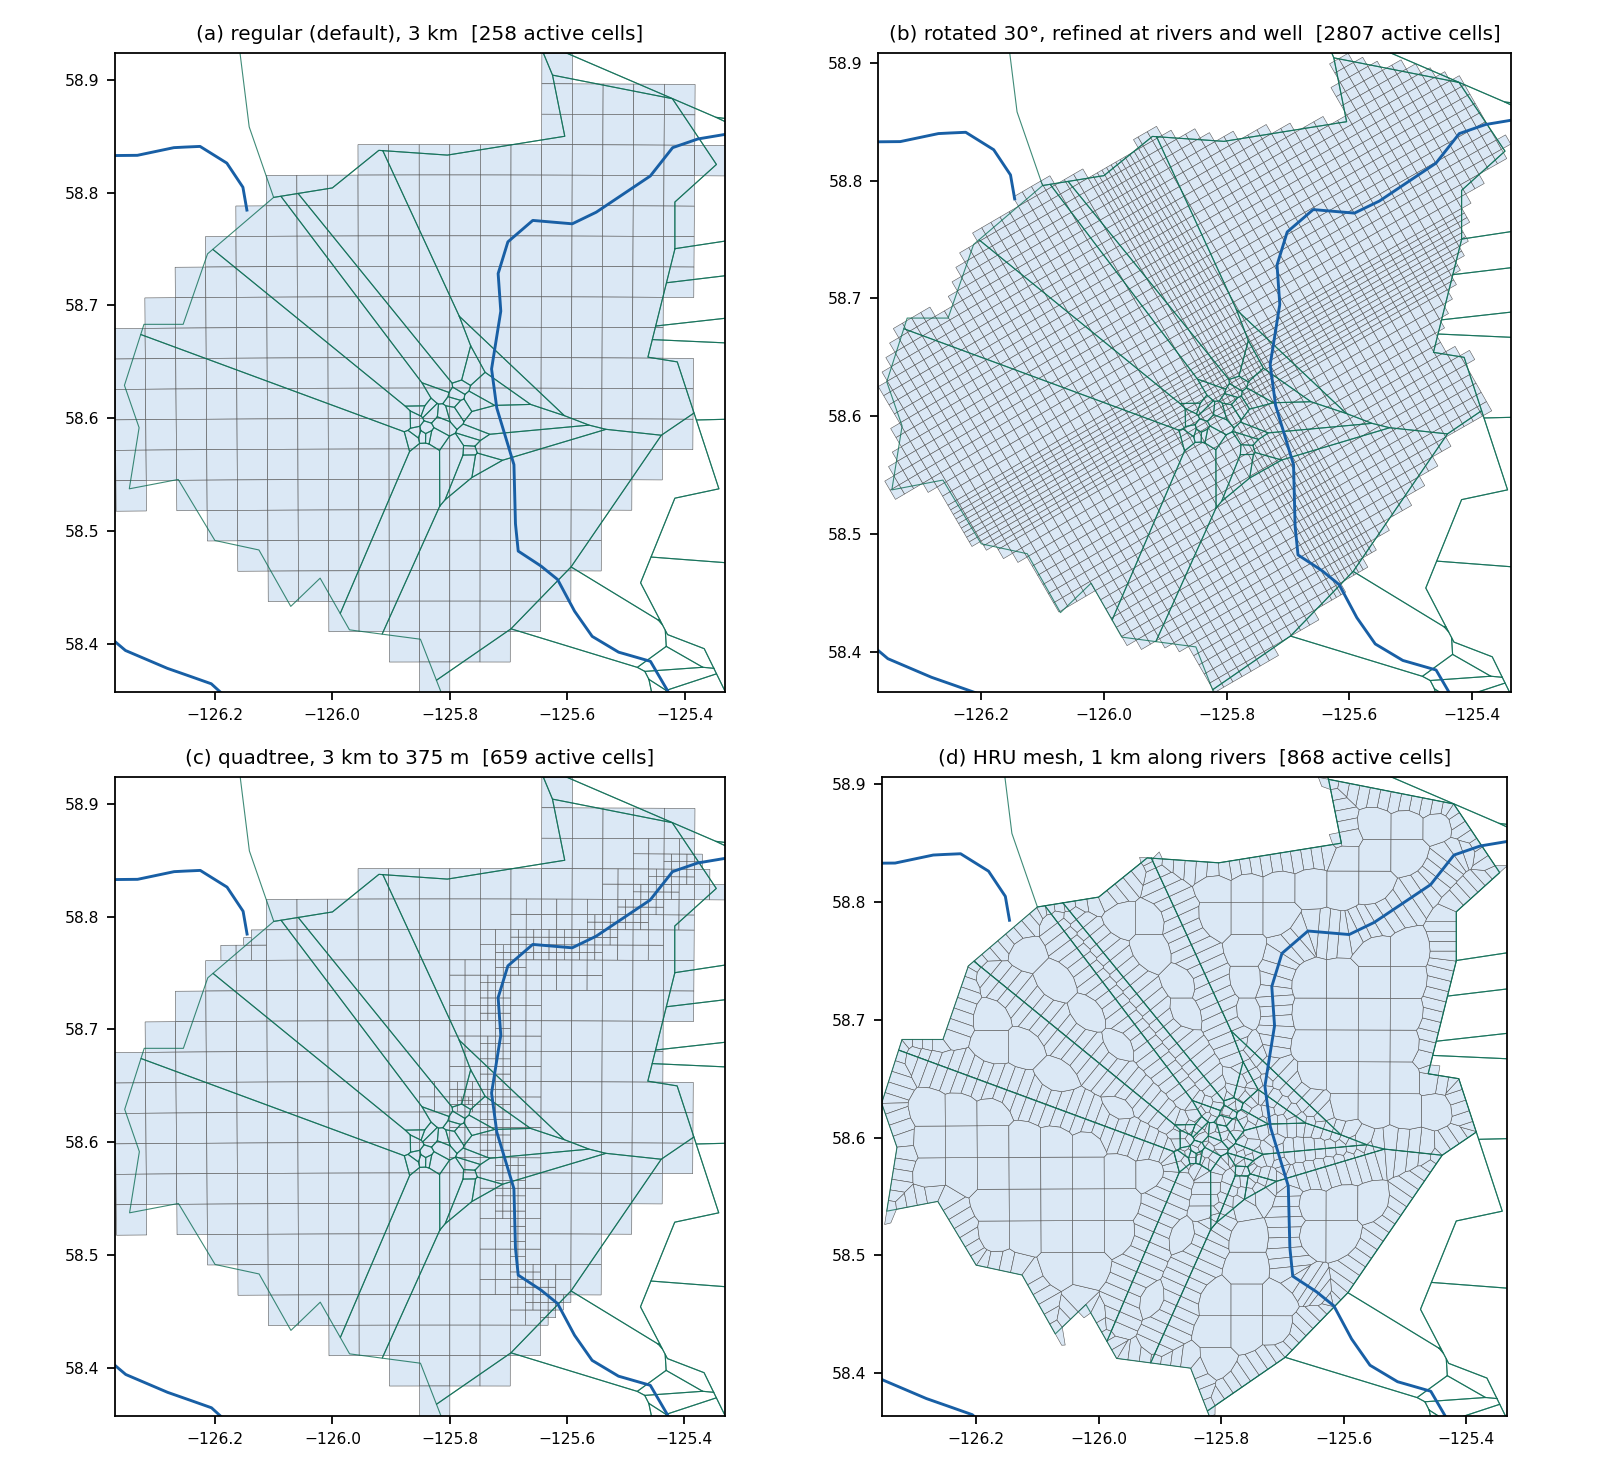
\includegraphics[width=0.78\linewidth]{figures/fig_grids.png}
\caption{The same model (Liard subbasin 52, HRU boundaries green, rivers blue) on four grids: (a) the default regular
grid; (b) rotated 30\textdegree{} and refined along rivers and around a well; (c) a quadtree refined along rivers and around the
well; (d) an HRU mesh whose cells follow HRU boundaries, with cells along the rivers.}\label{fig:grids}
\end{figure}

\subsection{Regular grids: rotation and variable spacing}
\cmd{:GridRotation} $\theta$ turns the grid $\theta$ degrees counterclockwise, for example to align columns with a valley.
The grid is built in its own rotated frame, in which every cell is still a rectangle; HRU polygons, rivers, wells and
boundaries are rotated into that frame, and MODFLOW receives the rotation as \cmd{ANGROT}. With \cmd{:GridRefinement} the grid gets variable spacing. Every base column and row that comes within the target size of a
refinement feature is divided into equal parts no larger than the target. Neighbouring columns and rows are then halved
until the widths change by at most a factor of two from one to the next. Refinement therefore always spans whole columns and rows.

\subsection{Quadtree grids}
A quadtree starts from large squares and cuts a square into four smaller ones wherever finer detail is wanted --- along a
river, say --- repeating until the cells are small enough. With \cmd{:GridType QUADTREE} a square is split into four while it is larger than the target size and a refinement feature
lies within half the target size of it. Splitting stops after \cmd{:QuadtreeMaxLevel} halvings (by default, enough to
reach the smallest target). The tree is then balanced so that neighbouring cells differ by one level at most. Where a large cell meets two
small ones its side carries the extra corner of the small cells (a hanging vertex), so MODFLOW's DISV input finds every
shared face. Because the line joining the centres of a large and a small cell is not perpendicular to their shared face,
MODFLOW's XT3D correction (the full conductance tensor) could be used. It is off by default, for two reasons found in the tests of Chapter~\ref{ch:verification}. The balanced quadtree was as
accurate without it (Thiem test). And XT3D --- even in its right-hand-side form --- slowed the Newton method badly where cells
dry and rewet: on the Liard model it took 32 instead of 7 iterations per day, and some days failed. \cmd{:FlowCorrection XT3D\_RHS} or \cmd{XT3D} switch it on.

\subsection{Meshes that follow HRU boundaries}
Picture a dot for every cell: each cell is the area closer to its own dot than to any other dot (a \emph{Voronoi} cell). If
two dots sit on opposite sides of an HRU boundary, at the same distance from it, the edge between their cells falls exactly
on that boundary. Raven places its dots this way, so the cells follow the HRU boundaries. In detail, with
\cmd{:GridType HRU\_MESH} the seed points are:
\begin{enumerate}
\item along every HRU boundary, pairs of seeds mirrored across the boundary at spacing $\delta_b=\min(\Delta/2,$ smallest
line refinement size (\cmd{RIVERS}, \cmd{LINES})$)$, or the \cmd{LAKES}/\cmd{POLYGONS} size where the boundary passes within
one such size of a refinement polygon, and $0.3\,\delta_b$ from it --- the face between the two seeds of a pair lies on the boundary;
\item seeds along refinement lines (rivers run through cell centres), in rings around refinement points (wells), and on a
staggered lattice of the target size inside and within one size around refinement polygons (lakes); seeds outside the
model's box (e.g.\ a monitoring well outside the model) are left out;
\item interior seeds on a lattice of spacing $\Delta$, kept only where no other seed is closer than about half the spacing.
\end{enumerate}
Each cell is the part of the plane closer to its seed than to any other. Raven builds it by cutting away, for each
neighbouring seed, the half of the plane that is closer to that neighbour. Each face remembers the seed on its other side, so
the connections between cells are exact. The line joining two seeds crosses their shared face at right angles, which is the
arrangement MODFLOW's standard method assumes, so no XT3D is needed. Where boundaries meet at sharp corners a cell may cover slivers of two HRUs. The overlaps are computed exactly, as for any
other grid, so the water accounts are unaffected. \cmd{GWModelSummary.txt} reports how much of each active cell's area lies
in its main HRU (typically above 99\%).

\subsection{Imported cells}
With \cmd{:GridType FILE} and \cmd{:GridFile cells.geojson ID\_FIELD} the cells are the polygons of a GeoJSON file in
longitude/latitude or in the projection of \cmd{:InputCRS}, one single-ring polygon per cell, numbered by the ID field (default \cmd{CELL\_ID}). Cells may be
concave, and a cell side may be shared with several smaller cells (T-junctions): neighbours are found wherever edges of two
cells lie on the same line --- within 0.1\% of the edge length, because a straight edge drawn in one map projection bends
slightly in another --- and overlap. A face made of several pieces gets their total length and their average position and
direction. Repeated vertices, which GIS exports often contain, are removed first. MODFLOW receives the grid as DISU with the
connection lengths, face widths and face directions computed from the polygons. Imported cells need not be orthogonal; for strongly non-orthogonal cells consider
\cmd{:FlowCorrection XT3D\_RHS} and check the convergence in \cmd{GWBudget.csv}.

\subsection{Connecting layers by elevation}\label{sec:layerconn}
In a layered grid a cell connects sideways only to the cell with the same layer number. When neighbouring columns have
different profiles --- a gravel layer thinning out next to a till, say --- the same layer number can mean different
materials at different elevations. \cmd{:LayerConnection ELEVATION} writes the grid as DISU and connects every pair of
cells of neighbouring columns whose vertical intervals overlap, as staggered horizontal connections (MODFLOW's \cmd{IHC}
2), so water flows between the layers that actually touch. Pass-through cells are removed and the cells above and below
them connected directly.

\subsection{Refinement}
\begin{lstlisting}
:GridRefinement RIVERS   250                     # along :RiverGeometry lines
:GridRefinement WELLS    100                     # around pumping and monitoring wells
:GridRefinement LAKES    250                     # in and around every reservoir's lake HRU
:GridRefinement LINES    faults.geojson    200   # along any lines
:GridRefinement POLYGONS wetlands.geojson  250   # inside and around polygons
\end{lstlisting}
Sizes must be smaller than \cmd{:GridCellSize}. Refinement applies to regular (variable spacing), quadtree and HRU-mesh
grids; an imported grid is used as it is. A grid is limited to 5 million cells per layer: a cell size or refinement that
gives more stops the run before the grid is built, naming the command and the number of cells. An imported grid
(\cmd{:GridType FILE}) with more cells stops naming the file, and an HRU mesh whose refinement makes more seeds stops
naming \cmd{:GridRefinement}; the cell size cannot help there. For a regular grid the
count is exact: the refined columns and rows are counted with the 2:1 smoothing that adds cells around each refined
strip, as the build makes them (test N24). For a quadtree it is estimated level by level from the squares the refinement features touch, each square
counted once however many features touch it (overlapping or adjacent features add no more), plus about a fifth for the
2:1 balance: 6\% below the cells built on the Liard example's grids, and between a third below and a fifth above on small
test grids of lines and polygons. So the estimate stops the run only beyond 1.5 times the limit; a grid nearer the limit
is built, and the build stops once it passes the limit. An HRU mesh is estimated before its seeds are placed (pairs along
the HRU boundaries, which take seeds at the smallest \cmd{LINES} or \cmd{RIVERS} size, seeds along the lines, around the
points and over the polygons, and the interior lattice); it stops beyond 1.5 times the limit, or when the boundary seeds
are so close for the cell size that building the cells would take more than a few minutes (seeds every 0.1~m along
65~km of HRU boundaries with 500~m cells, a size meant in kilometres). A grid within the limit that still needs more
memory than the computer has stops with a message naming the command and the estimated size.

\cmd{LAKES} needs no extra file: the outline of the lake HRU of every Raven reservoir (\cmd{:Reservoir \dots\ :HRUID}) is taken
from \cmd{:HRUGeometry}. Fine cells around a lake place its seepage (\cmd{:ReservoirExchange}) and the exchange along its shore
more precisely. On a regular grid the rows and columns through the lake are refined; a quadtree splits the squares in and
near the lake; an HRU mesh places cells of the target size inside the lake and in a band one cell wide around it, and
shortens the spacing of its cells along the shore. \cmd{POLYGONS} works the same way for any outline in a file.

\subsection{Rivers and boundaries on any grid}
On the default grid each segment of a river or boundary line is cut into pieces of at most a twentieth of the cell size,
and each piece goes to the cell that holds its middle. On every other grid each piece of a line is cut exactly at the edges of the cells it crosses (rectangles along their
sides, other cells along their edges or triangle by triangle). River lengths per cell are therefore exact and do not
depend on the cell size. A stretch lying exactly on a shared cell edge
is counted once. A boundary line may be drawn along the edge of the modelled area, where the edge cells can be inactive because too little
of them is covered. Such a line is attached to the nearest active cell within one cell size, so a boundary drawn on the
watershed outline is never lost.

\subsection{Choosing a grid}
Start with the default grid and a cell size of a few kilometres. Refine where heads and exchanges change quickly: along
rivers that gain or lose much water, around pumping wells, around lakes and reservoirs that leak to the aquifer, and in
wetlands. A quadtree gives the most accuracy per cell;
an HRU mesh gives the cleanest HRU--cell linkage; a rotated regular grid is simplest when a valley has one direction. XT3D
(\cmd{:FlowCorrection XT3D\_RHS} or \cmd{XT3D}) is off by default; use it only for strongly non-orthogonal imported cells, and
check that the model still converges well.

\subsection{Grid outputs}
Every run writes \cmd{mf6/grid\_cells.geojson}: each cell as a longitude/latitude polygon with its number (as in MODFLOW and in
the hotstart file), whether it is active, its profile, its dominant HRU and its area --- ready to be joined with heads in
QGIS. For grids other than regular, \cmd{GWHeads.nc} has a \cmd{cell} dimension instead of rows and columns, and the hotstart
block is written as \cmd{:GWHeads} \emph{nlay} \cmd{1} \emph{ncells}. The grid type, cell sizes, MODFLOW format and HRU
fidelity are reported in \cmd{GWModelSummary.txt}. Setting the environment variable \cmd{RAVEN\_GW\_PROFILE=1} prints the time
taken by each stage of building the model, useful for large grids.

\section{Building the layers}\label{ch:layers}
\subsection{Land surface, model top and bedrock}
For each active column Raven needs three elevations:
\begin{description}
\item[Land surface] $z_{\mathrm{land},i}$: the average of 25 points ($5\times5$) of the DEM over the cell
(\cmd{:LandSurface}); without a DEM, the area-weighted \cmd{ELEVATION} of the HRUs in the cell.
\item[Model top] $z_{\mathrm{top},i}=z_{\mathrm{land},i}-d_{\mathrm{sz},a}$, where $d_{\mathrm{sz},a}$ is the
\cmd{SOIL\_ZONE\_DEPTH} of the column's profile $a=a(i)$ (default 0, so the top is the land surface). With the soil-zone
coupling (\cmd{:SoilZone PHYSICAL}, Section~\ref{ch:soilzone}) \cmd{SOIL\_ZONE\_DEPTH} is ignored for HRUs with a soil zone: the soil-zone thickness
is the sum of the listed soil layers.
\item[Bedrock] $z_{\mathrm{br},i}$: the average of 25 points of the bedrock map (\cmd{:BedrockSurface}); without a map,
$z_{\mathrm{land},i}-D_a$ with $D_a$ the profile's \cmd{DEFAULT\_BEDROCK\_DEPTH}.
\end{description}
A column whose bedrock lies less than 0.5 m below its top has no room for an aquifer and is made inactive.

\subsection{Stacking the layers}
A profile lists its layers from the top down, each with a material (\emph{aquifer class}), a thickness $b_\ell$ (or
\cmd{TO\_BEDROCK}) and a type. The bottom of layer $\ell$ is
\begin{equation}
z^{(\ell)}_{\mathrm{bot},i}=
\begin{cases}
z_{\mathrm{br},i} & \text{for a \cmd{TO\_BEDROCK} layer,}\\
\max\!\left(z^{(\ell-1)}_{\mathrm{bot},i}-b_\ell,\;z_{\mathrm{br},i}\right) & \text{otherwise,}
\end{cases}
\qquad z^{(0)}_{\mathrm{bot},i}\equiv z_{\mathrm{top},i}.
\end{equation}
Layers never extend below bedrock. Two special cases:
\begin{itemize}
\item A layer (other than the first) cut to less than 0.5 m by bedrock becomes a \emph{pass-through} cell: it is given
a nominal thickness of 0.01 m and MODFLOW's \cmd{IDOMAIN}~$=-1$, which removes it from the calculation while
connecting the cells above and below it directly.
\item The model has as many layers as the thickest profile. Where a profile has fewer layers, the missing ones are
pass-through cells.
\end{itemize}

\begin{example}[: one column]
Land surface 600 m, bedrock 555 m, profile \cmd{VALLEY\_ALLUVIUM} = gravel 15 m, clay till 5 m, sand \cmd{TO\_BEDROCK}.
Top = 600 m. Layer 1 (gravel): bottom $\max(600-15,555)=585$ m. Layer 2 (till): bottom $\max(585-5,555)=580$ m.
Layer 3 (sand): bottom 555 m (to bedrock), thickness 25 m. If bedrock were at 582 m instead, layer 2 would end at
$\max(580,582)=582$ m (3 m thick), and layer 3, which runs to bedrock, would span 582 to 582 m --- zero thickness, so it becomes
a pass-through cell.
\end{example}

\begin{figure}[!htbp]\centering
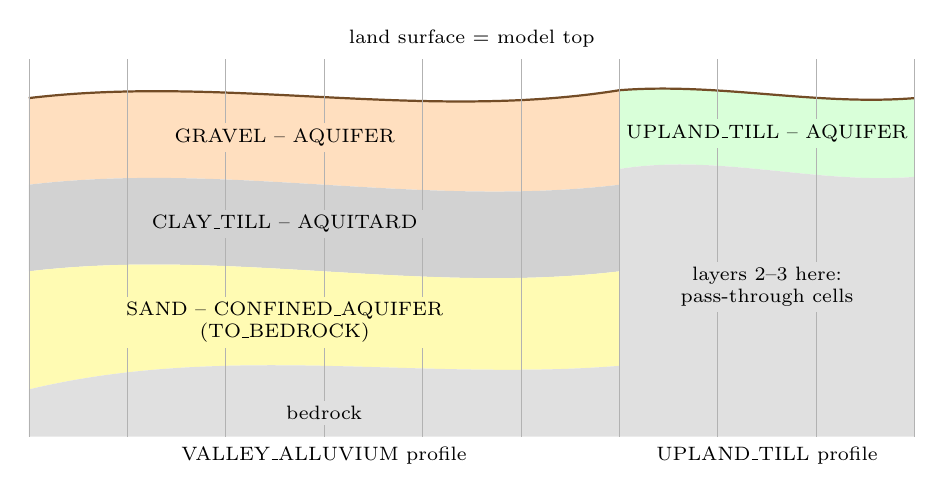
\begin{tikzpicture}[x=1.25cm,y=1.0cm,lab/.style={font=\scriptsize,align=center,inner sep=2pt}]
\fill[orange!25] (0,4.3) .. controls (2,4.6) and (4,4.0) .. (6,4.4) -- (6,3.2) .. controls (4,2.9) and (2,3.5) .. (0,3.2) -- cycle;
\fill[gray!35] (0,3.2) .. controls (2,3.5) and (4,2.9) .. (6,3.2) -- (6,2.1) .. controls (4,1.8) and (2,2.4) .. (0,2.1) -- cycle;
\fill[yellow!30] (0,2.1) .. controls (2,2.4) and (4,1.8) .. (6,2.1) -- (6,0.9) .. controls (4,0.7) and (2,1.2) .. (0,0.6) -- cycle;
\fill[black!12] (0,0.6) .. controls (2,1.2) and (4,0.7) .. (6,0.9) -- (6,0) -- (0,0) -- cycle;
\fill[green!15] (6,4.4) .. controls (7,4.5) and (8,4.2) .. (9,4.3) -- (9,3.3) .. controls (8,3.2) and (7,3.6) .. (6,3.4) -- cycle;
\fill[black!12] (6,0) -- (6,3.4) .. controls (7,3.6) and (8,3.2) .. (9,3.3) -- (9,0) -- cycle;
\draw[thick,brown!60!black] (0,4.3) .. controls (2,4.6) and (4,4.0) .. (6,4.4) .. controls (7,4.5) and (8,4.2) .. (9,4.3);
\foreach \x in {0,1,...,9} \draw[gray!60,very thin] (\x,0) -- (\x,4.8);
\node[lab,fill=white,inner sep=1pt] at (4.5,5.05) {land surface = model top};
\node[lab,fill=orange!25] at (2.6,3.8) {GRAVEL -- \cmd{AQUIFER}};
\node[lab,fill=gray!35] at (2.6,2.7) {CLAY\_TILL -- \cmd{AQUITARD}};
\node[lab,fill=yellow!30] at (2.6,1.45) {SAND -- \cmd{CONFINED\_AQUIFER}\\ (\cmd{TO\_BEDROCK})};
\node[lab,fill=black!12] at (3.0,0.3) {bedrock};
\node[lab,fill=green!15] at (7.5,3.85) {UPLAND\_TILL -- \cmd{AQUIFER}};
\node[lab,fill=black!12] at (7.5,1.9) {layers 2--3 here:\\ pass-through cells};
\node[lab,anchor=north] at (3,-0.05) {\cmd{VALLEY\_ALLUVIUM} profile};
\node[lab,anchor=north] at (7.5,-0.05) {\cmd{UPLAND\_TILL} profile};
\end{tikzpicture}
\caption{Layers are stacked from the model top and clipped at bedrock; the one-layer upland profile is padded with
pass-through cells.}\label{fig:layers}
\end{figure}

\subsection{Layer types}
\begin{table}[!htbp]\centering
\caption{Layer types.}\label{tab:types}\small
\begin{tabular}{P{0.31\linewidth}P{0.27\linewidth}P{0.348\linewidth}}\toprule\hdr
Type in the profile & MODFLOW 6 setting & What it means\\\midrule
\cmd{AQUIFER} (\cmd{UNCONFINED\_AQUIFER}) & \cmd{ICELLTYPE}=1, \cmd{ICONVERT}=1 & water table can be inside the layer: storage by $S_y$, transmissivity from the saturated thickness\\
\cmd{CONFINED\_AQUIFER} & \cmd{ICELLTYPE}=0, \cmd{ICONVERT}=0 & always full: constant transmissivity, storage by $S_s$\\
\cmd{AQUITARD} & as \cmd{AQUIFER}, with the low $K$ of its class & slow leaky layer, simulated explicitly\\
\cmd{AQUICLUDE} & \cmd{IDOMAIN}=0 & no flow at all through this layer (not allowed as the top layer)\\\bottomrule
\end{tabular}
\end{table}

\subsection{Material properties}
Each layer takes its properties from its aquifer class (\cmd{:AquiferClasses}): horizontal conductivity $K_h$
(\cmd{K\_HORIZ}), vertical conductivity $K_v$ (\cmd{K\_VERT}, default $K_h/10$), $S_s$ (\cmd{SPEC\_STORAGE}, default
$10^{-5}$), $S_y$ (\cmd{SPEC\_YIELD}, default 0.1) and porosity (\cmd{POROSITY}, default 0.3; stored for future transport
calculations; MODFLOW's flow calculation does not use it).

\begin{watch}
By default (\cmd{:LayerConnection INDEX}) MODFLOW connects layer $\ell$ of one column sideways only to layer $\ell$ of its
neighbours. Where two profiles meet, list their layers in the same geological order, otherwise, for example, a gravel layer
may connect to a clay layer; or use \cmd{:LayerConnection ELEVATION} (Section~\ref{sec:layerconn}), which connects the
cells whose elevations overlap. (An existing model keeps its own connections.)
\end{watch}

\subsection{Initial heads}
The starting head of every cell in a column is
\begin{equation}
h^0_i=\max\!\left(z_{\mathrm{land},i}-d_0,\;z_{\mathrm{low},i}+0.1\right),
\end{equation}
where $d_0$ is the profile's \cmd{INITIAL\_HEAD\_DEPTH} (or the value given by \cmd{:InitialGWHeads} in the \cmd{.rvc}
file), and $z_{\mathrm{low},i}$ is the bottom of the lowest active cell. With \cmd{:InitialGWHeads ELEVATION z}, $z$ replaces $z_{\mathrm{land},i}-d_0$ (still at least 0.1 m above the lowest active cell bottom).
A hotstart (\cmd{:GWHeads} in the \cmd{.rvc}) overrides all of this cell by cell. Optionally, a steady-state
calculation replaces these first guesses (Section~\ref{sec:init}).
When $d_0$ is larger than the layers above the water table are thick, a whole layer can start dry. Raven checks this at
start-up (cold start without a steady-state period, or hotstart heads): a layer whose active convertible cells all start at
or below their bottom gets one warning naming the layer and a line ``dry at the start'' in \cmd{GWModelSummary.txt}.
MODFLOW then has to rewet the whole layer in the first steps, which can take many iterations or leave some of them
unconverged; start from \cmd{:GWInitialization STEADY\_STATE}, a smaller \cmd{INITIAL\_HEAD\_DEPTH} or
\cmd{:InitialGWHeads}. Confined layers (\cmd{CONFINED\_AQUIFER}) never dry and are not checked.

\subsection{The generated MODFLOW files}
Raven writes a standard MODFLOW~6 simulation to \cmd{<output>/mf6/}: \cmd{mfsim.nam} (simulation), \cmd{sim.tdis}
(time steps), \cmd{sim.ims} (solver), \cmd{gwf.nam} (model), \cmd{gwf.dis} (grid), \cmd{gwf.npf} (conductivities and
layer types), \cmd{gwf.sto} (storage), \cmd{gwf.ic} (initial heads), \cmd{gwf.oc} (output control) and one file per
exchange package (\cmd{gwf.rch}, \cmd{gwf.drn}, \cmd{gwf.riv}, \cmd{gwf.evt}, \cmd{gwf.wel}, \cmd{gwf.ghb}, \cmd{gwf.chd},
\cmd{gwf.swx}, \cmd{gwf.res}). Grid arrays are written layer by layer, each grid row starting on a new line, which is
how MODFLOW reads them. These files can be opened in FloPy or ModelMuse; they never need editing.

\section{Parameters for building the model}\label{sec:buildparams}
The grid and layers are built from the following parameters; the class column says where each is set, the reference column
where its default and allowed range are listed.
\begin{table}[!htbp]\centering
\caption{Parameters for building the model.}
\begin{tabular}{>{\raggedright\arraybackslash}P{0.09\linewidth}>{\raggedright\arraybackslash}P{0.26\linewidth}>{\raggedright\arraybackslash}P{0.287\linewidth}>{\raggedright\arraybackslash}P{0.1\linewidth}>{\raggedright\arraybackslash}P{0.15\linewidth}}\toprule\hdr
Symbol & Parameter & Class (where it is set) & Units & Reference\\\midrule
$\Delta$ & \cmd{:GridCellSize} & \cmd{.rvg} option & m & Sec.~\ref{app:commands}\\
$f_{\min}$ & \cmd{:MinCellCoverage} & \cmd{.rvg} option & -- & Sec.~\ref{app:commands}\\
-- & \cmd{AQUIFER\_PROFILE} & HRU attribute (\cmd{:HRUs}, \cmd{.rvh}) & -- & Sec.~\ref{app:commands}\\
$P_k$ & HRU polygon & \cmd{:HRUGeometry} (\cmd{.rvg}) & -- & Sec.~\ref{app:commands}\\
$z_{\mathrm{land}}$ & land surface & \cmd{:LandSurface} (\cmd{.rvg}); else HRU \cmd{ELEVATION} & m & Sec.~\ref{app:commands}\\
$z_{\mathrm{br}}$ & bedrock & \cmd{:BedrockSurface} (\cmd{.rvg}); else \cmd{DEFAULT\_BEDROCK\_DEPTH} (aquifer profile) & m & Sec.~\ref{app:profile}\\
$d_{\mathrm{sz},a}$ & \cmd{SOIL\_ZONE\_DEPTH} & aquifer profile $a$ & m & Sec.~\ref{app:profile}\\
$b_\ell$ & layer thickness, type & aquifer profile (\cmd{:AquiferProfiles}) & m & Sec.~\ref{app:layers}\\
$K_h$, $K_v$ & \cmd{K\_HORIZ}, \cmd{K\_VERT} & aquifer class of the layer & m/d & Sec.~\ref{app:class}\\
$S_s$, $S_y$ & \cmd{SPEC\_STORAGE}, \cmd{SPEC\_YIELD} & aquifer class of the layer & 1/m, -- & Sec.~\ref{app:class}\\
$d_0$ & \cmd{INITIAL\_HEAD\_DEPTH}; \cmd{:InitialGWHeads} & aquifer profile; \cmd{.rvc} & m & Sec.~\ref{app:profile}\\
\bottomrule
\end{tabular}
\end{table}

\section{What the generated files look like}
The model name file lists the packages Raven uses:
\begin{lstlisting}
BEGIN OPTIONS
  NEWTON
END OPTIONS
BEGIN PACKAGES
  DIS6  gwf.dis  DIS
  NPF6  gwf.npf  NPF
  STO6  gwf.sto  STO
  IC6   gwf.ic   IC
  RCH6  gwf.rch  RCH_RAVEN
  DRN6  gwf.drn  DRN_RAVEN
  RIV6  gwf.riv  RIV_RAVEN
  OC6   gwf.oc   OC
END PACKAGES
\end{lstlisting}
The grid file records the projection in its first line, so the grid can be placed on a map:
\par\noindent\begin{minipage}{\linewidth}
\begin{lstlisting}
# Lambert azimuthal equal-area projection, origin lat=58.81662353 lon=-125.4914706 (sphere R=6371007.181 m)
BEGIN DIMENSIONS
  NLAY 3
  NROW 85
  NCOL 54
END DIMENSIONS
\end{lstlisting}
\end{minipage}\par\smallskip
Boundary packages contain one line per cell with placeholder values; Raven replaces the values in memory every step, so
the files show the grid positions of recharge, drains, rivers, wells and boundaries but not their daily values.

\section{Solver settings}
Why such a small head tolerance? MODFLOW stops iterating when no head changes by more than the tolerance, but a flow is a
conductance times a head difference. The seepage drains have very large conductances (one 1 km cell with a leakance of
1~d$^{-1}$ has $10^6$~m$^2$/d), so a head tolerance of 1 cm could still leave about $10^4$~m$^3$/d of imbalance in such a cell on a
difficult day. With 0.01 mm the imbalance is a thousand times smaller than with 1 cm. The price is more Newton iterations --- in the
20-year Liard run about 10 per day on average instead of 7--8 --- and a run about twice as long. The value was chosen from the
randomized tests: at 0.1 mm a few extreme set-ups (drain conductance $2\times10^7$~m$^2$/d per cell) still showed a 0.2\%
residual on single steps; at 0.01 mm none did.

\paragraph{Two-tier convergence.} A very tight tolerance can occasionally stall the Newton iterations on a hard step. The target is the tolerance above. If a step has not reached it after 100 iterations (or half the iteration limit, if that is smaller), the coupler raises
MODFLOW's own tolerance to ten times the target (0.1 mm) for the rest of that step only, and restores it for the next step. MODFLOW's own test always decides whether a step has converged. A step accepted at the relaxed tolerance is therefore as
reliable as a step of a model run with that tolerance. Only if even that fails within the iteration limit is the step
reported as not converged. \cmd{GWBudget.csv} records which
case applied (\emph{converged} = 1 target reached, 2 accepted at the relaxed tolerance, 0 not converged).
The water exchanged between Raven and MODFLOW is exact at any tolerance --- both sides use the same computed flows ---
so the tolerance only controls MODFLOW's own small numerical residual.

\begin{table}[!htbp]\centering
\caption{MODFLOW solver settings (\cmd{sim.ims}).}
\begin{tabular}{P{0.36\linewidth}P{0.14\linewidth}P{0.428\linewidth}}\toprule\hdr
IMS setting & Value & Meaning\\\midrule
\cmd{COMPLEXITY} & \cmd{COMPLEX} & robust defaults for non-linear problems\\
\cmd{OUTER\_DVCLOSE} & 0.00001 m & Newton iterations stop when no head changes by more than this (\cmd{:SolverHead\allowbreak Tolerance})\\
\cmd{OUTER\_MAXIMUM} & 500 & iteration limit (\cmd{:SolverMax\allowbreak OuterIterations})\\
\cmd{UNDER\_RELAXATION} & \cmd{DBD} & damps oscillating head changes (theta 0.7, kappa 0.07, gamma 0.1)\\
\cmd{BACKTRACKING\_NUMBER} & 20 & retries with a smaller step when the imbalance grows\\
\cmd{INNER\_MAXIMUM} & 500 & linear-solver iteration limit\\
\cmd{INNER\_DVCLOSE}, \cmd{INNER\_RCLOSE} & $0.1\times$ outer, 1 m$^3$/d & linear-solver tolerances\\
\cmd{LINEAR\_ACCELERATION} & \cmd{BICGSTAB} & linear solver\\
\cmd{PRECONDITIONER\_LEVELS} & 5 & ILU fill level\\\bottomrule
\end{tabular}
\end{table}

\section{How MODFLOW solves each time step}\label{ch:mf6}
\subsection{Time steps}
MODFLOW's time steps are generated from Raven's \cmd{:StartDate}, \cmd{:Duration} ($t_{\mathrm{end}}$) and \cmd{:TimeStep} ($\dt$): one transient
stress period of $N=\mathrm{round}(t_{\mathrm{end}}/\dt)$ steps of length $\dt$, preceded by a one-day steady-state period when
\cmd{:GWInitialization STEADY\_STATE} is used. MODFLOW therefore always takes exactly one step for each Raven step.
If Raven would run more steps than MODFLOW holds, Raven stops with a clear message.

\subsection{Cells that dry and rewet: the Newton method}
An unconfined cell whose water table falls below its bottom is \emph{dry}. Older MODFLOW versions switched such cells
off, which often made the solution fail when they needed to switch back on. MODFLOW~6's Newton--Raphson method, which the coupling always uses, keeps dry cells in the calculation. The conductance
between two cells is scaled smoothly by how full the upstream cell is, and falls to zero as that cell empties. The cell
fills again naturally when water arrives. The solver settings written by Raven are:
\begin{itemize}
\item outer (Newton) iterations up to 500 (\cmd{:SolverMax\allowbreak OuterIterations}), head-change tolerance 0.00001 m (\cmd{:SolverHead\allowbreak Tolerance});
\item delta-bar-delta under-relaxation (damps oscillating head changes) and backtracking (retries a smaller change
when the residual grows);
\item inner linear solver BiCGSTAB with an ILU preconditioner of level 5, residual tolerance 1.0 m$^3$/d.
\end{itemize}
The Newton option is written without its own \cmd{UNDER\_RELAXATION} keyword, which resets a head that falls below the cell
bottom. With MODFLOW~6.6 that reset made the Newton change of a drying cell repeat unchanged at every iteration, so the
step never converged (on the Liard model this happened on most days once the thin aquitard under the gravel began to dry).
Without it, MODFLOW~6.6.3 and 6.8.1 converge in the same few iterations.
Raven runs the Newton iterations itself through MODFLOW's interface (prepare, repeated solve, finalize), so it knows
whether each step converged. If a step does not converge, MODFLOW continues (option \cmd{CONTINUE}), the step is
flagged in \cmd{GWBudget.csv}, and a safeguard limits what that step can return to Raven (Section~\ref{sec:guard}).

\subsection{Connectivity between aquifer areas}
Because dry cells carry no flow, parts of an aquifer can become disconnected when the water table falls and join
again when it rises, without any action by the user. Streams disconnect from a falling water table in the same way
(Section~\ref{ch:rivers}). To show this, \cmd{GWConnectivity.csv} reports each step:
\begin{itemize}
\item the fraction of top-layer cells of each profile that are \emph{wet}, meaning $h_i>z^{(1)}_{\mathrm{bot},i}+10^{-3}$ m;
\item the number of separate wet areas, where two wet cells belong to the same area if they share an edge
(4-neighbour connectivity; counted by a flood-fill of the wet cells).
\end{itemize}
This is a diagnostic only; it does not affect the calculation.

\subsection{Heads of dry cells}
Under the Newton method a dry cell carries no flow, and MODFLOW leaves its head at whatever value the solver reaches; it
can be far below the cell bottom (values of $-10^{8}$~m have been seen in a pumped, isolated cell). MODFLOW's own flows are
unaffected, but such a head is not a water level. Wherever the coupling needs a real water level it therefore uses the \emph{water table} of the column: the head of the
highest cell whose head is above its bottom, or the bottom of the lowest active cell if all are dry. This is used for the
reservoir's local groundwater level, in \cmd{GWHRUState.csv}, and for monitoring wells (a well screened in a dry cell
reports a missing value, \cmd{-1.2345}). The MODFLOW head file and the hotstart heads keep
MODFLOW's raw values, so a restart continues exactly.
